\section{Linear/Circular Accelerators, Solutions for Continuous Sources}

\subsection{Linear/Circular Accelerators}
Last time we derived the generalization of the Larmor formula:
\begin{equation}
    P = \frac{q^2\mu_0}{6\pi c}\gamma^6\left[\abs{\dot{\v{v}}}^2 - \left(\frac{\v{v} \times \dot{\v{v}}}{c}\right)^2\right]_{\text{ret}}
\end{equation}
with $\gamma = \frac{1}{\sqrt{1- \frac{\abs{\v{v}}^2}{c^2}}}$ the familiar Lorentz factor. Let us study the two cases:
\begin{itemize}
    \item $\v{v} \parallel \dot{\v{v}}$ (relevant for linear accelerators). In this case, we have that $\v{v} \times \dot{\v{v}} = \v{0}$, so the formula simplifies to:
    \begin{equation}\label{eq:powerparallel}
        P = \frac{q^2\mu_0}{6\pi c}\gamma^6\abs{\dot{\v{v}}}^2
    \end{equation}

    The structures appearing here can be naturally written in terms of the change in (relativistic) momentum $p = m\gamma v$:
    \begin{equation}
        \dod{p}{t} = m\dod{}{t}(\gamma v) = m\dod{}{t}\left(\frac{v}{\sqrt{1 - \frac{v^2}{c^2}}}\right) = m\gamma^3\dot{v}
    \end{equation} 
    We can thus write Eq. \eqref{eq:powerparallel} in terms of the rate of change of momentum:
    \begin{equation}
        P = \frac{q^2\mu_0}{6\pi c m^2}\left(\dod{p}{t}\right)^2
    \end{equation}
    How do we interpret this? Well, recall the particle satisfies the dispersion relation:
    \begin{equation}
        E^2 = p^2c^2 + (mc^2)^2 = m \gamma c^2
    \end{equation}
    We find from the above that, in the linear case:
    \begin{equation}
        \dod{p}{t} = \dod{E}{x}
    \end{equation}
    where we parametrize the particle energy at position $E(x)$. If we make this replacement:
    \begin{equation}
        P = \frac{q^2\mu_0}{6\pi c m^2}\left(\dod{E}{x}\right)^2
    \end{equation}
    This is much more visual. The whole reason why we made this accelerator is to accelerate particles, and we only have a finite amount of real estate to do this. We therefore want the rate of change of the energy of the particle to be as large as possible. But then we pay the price in radiation\footnote{There is no such thing as a free lunch. There is such a thing as a very expensive lunch.}.

    \item $\v{v} \perp \dot{\v{v}}$ (relevant for circular accelerators). In this case, the cross product of the velocity/acceleration is just the product of the magnitudes, so $\abs{\v{v} \times \dot{\v{v}}}^2 = \abs{\v{v}}^2\abs{\dot{\v{v}}}^2$ and so:
    \begin{equation}
        P = \frac{q^2\mu_0}{6\pi c}\gamma^4\abs{\dot{\v{v}}}^2
    \end{equation}
    Compare the $\gamma^4$ to the $\gamma^6$ for the linear accelerators. But, in the circular case, we pay the price of $\gamma^4$ even if the particle does not accelerate - it costs energy to just keep the particle moving around. In particular, we can ask - how much energy is lost per revolution\footnote{One time around the circle, not the communist revolution}?

    For radius $\rho$, can write the period as:
    \begin{equation}
        T = \frac{2\pi \rho}{v} = \frac{2\pi \rho}{c\beta}
    \end{equation}
    the acceleration is then:
    \begin{equation}
        a = \frac{v^2}{\rho}
    \end{equation}
    And we find:
    \begin{equation}
        \Delta E = TP = \frac{1}{3}q^2\mu_0 \gamma^4\frac{v^3}{\rho}
    \end{equation}
    In the LHC, the charged particles are protons, and the radius is $\rho \sim 27\si{km}$. The mass of the protons are:
    \begin{equation}
        m_P c^2 \sim 1\si{GeV}
    \end{equation}
    The energies the protons are accelerated to are:
    \begin{equation}
        E \sim 10\si{TeV} = 10000\si{GeV}
    \end{equation}
    So:
    \begin{equation}
        E = m_p \gamma c^2 \implies \gamma = \frac{E}{m_p c^2} = 10000
    \end{equation}
    In this limit, $v \sim c$ and so:
    \begin{equation}
        \Delta E = \frac{1}{3}q^2\mu_0 \gamma^4\frac{c^3}{\rho} \sim 2.2\si{keV}
    \end{equation}
    Note that this is \emph{not} the energy lost to radiation while accelerating the protons, but rather the energy lost per revolution after they are already brought up to speed. You might say that the 2.2keV looks puny in comparison to the 10TeV energy. But you have to remember that every second, the protons do 10000 revolutions. Therefore, each second we lose 22MeV, and we must inject this amount of energy if we do not want the protons to slow down. This operates 8-10 hours a day, and there is more than 1 proton in the system... it is not our job here, but if you go into designing accelerators in the future, this is something you will need to think about.
    \end{itemize}

\begin{center}
    \emph{End of midterm content.}
\end{center}

\subsection{Solving Maxwell for continuous sources}
Consider now the continuous distributions $\rho(\v{x}, t), \v{J}(\v{x}, t)$. The question we want to discuss is simple - somebody hands you the above, and you want to solve the Maxwell equations with these sources. A good discussion of the 

A couple comments:
\begin{itemize}
    \item We are dealing with linear differential equations, and thus the general solution with a given source $J^\mu(x)$ is the same as any particular solution $A_\mu^{p}(x)$ with the source + the general solution of the homogenous equation/source-free case $A_\mu^{\text{free}}(x)$.
    \item If $A_\mu^{(1)}$ is a solution for source $J_\mu^{(1)}$ and $A_\mu^{(2)}$ is a solution for source $J_\mu^{(2)}$, then $A_\mu^{(1)} + A_\mu^{(2)}$ is a solution for source $J_\mu^{(1)} + J_\mu^{(2)}$.
\end{itemize}
These two observations simplifies things considerably. Namely, it suffices to consider:
\begin{equation}
    \rho(\v{x}, t) \stackrel{?}{=} \rho(\v{x})\exp(-i\omega t)
\end{equation}
There are some points to make. First, the $\rho$s appearing on different sides of the equation are different functions, but we will have to accept such abuse of notation. Second, the RHS is complex, so we really have to take the real part:
\begin{equation}
    \rho(\v{x}, t) = \Re(\rho(\v{x})\exp(-i\omega t))
\end{equation}
Back to the central point - why can we generically write things this way? Well, consider the Fourier transform:
\begin{equation}
    \rho(\v{x}, t) = \frac{1}{2\pi}\int d\omega \tilde{\rho}(\v{x}, \omega)e^{i\omega t}
\end{equation}
then the fact that we can take linear superpositions of solutions tells us that it suffices to look at $\Re(\rho(\v{x})\exp(-i\omega t))$. Similarly, we consider:
\begin{equation}
    \v{J}(x) = \v{J}(\v{x}, t) = \Re(\v{J}(\v{x})e^{-i\omega t})
\end{equation}
If we plug these into the continuity equation:
\begin{equation}
    \p_t \rho + \nabla \cdot \v{J} = 0
\end{equation}
then:
\begin{equation}
    i\omega \rho(\v{x}) = \nabla \cdot \v{J}(\v{x})
\end{equation}

We can now obtain the vector potential:
\begin{equation}
    \v{A}(x) = \frac{\mu_0}{4\pi}\int d^4x' \frac{\v{J}(x')}{\abs{\v{x} - \v{x}'}}\delta(t' - t + \frac{\abs{\v{x} - \v{x}'}}{c})
\end{equation}
And analogous for $\phi$. We remark that this vanishes if $\v{J} = \v{0}$, which is not true for the general solution - it is just a particular solution. When we write down the above, we are fixing the freedom in $\v{A}$, and saying that we are only interested in the vector potential that arises from the sources of interest.

The time part of the integral is very simple, because we only get a contribution from the delta function:
\begin{equation}\label{eq:Aintegral}
    \v{A}(\v{x}) = \frac{\mu_0}{4\pi}\int d^3\v{x}'\v{J}(\v{x}')\frac{e^{ik\abs{\v{x} - \v{x}'}}}{\abs{\v{x} - \v{x}'}}
\end{equation}
with $k = \omega/c$. We have also made the same replacement that $\v{A}(x) = \v{A}(\v{x})e^{-i\omega t}$ in the above so the dependence drops out. Now writing down the field:
\begin{equation}
    \v{H} = \frac{1}{\mu_0}\v{B} = \frac{1}{\mu_0}\nabla \times \v{A} 
\end{equation}
and $\v{E}$ we obtain as:
\begin{equation}
    \v{E} = \frac{iZ_0}{k}\nabla \times \v{H}
\end{equation}
with:
\begin{equation}
    Z_0 = \sqrt{\frac{\mu_0}{\e_0}}
\end{equation}
the impedance of the vacuum.

Presumably, there is some finite region in space where the source $J^\mu$ is nonzero. The integral over $\v{x}'$ in Eq. \eqref{eq:Aintegral} therefore is actually over a finite region. One scale that appears is $d$ (the size of the distribution) and another is the wavelength $\lambda = \frac{2\pi}{k}$, which governs the length over which the exponent varies. Finally, there is a third scale $r = \abs{\v{x}}$ which is the distance from the source to the detector.

\begin{center}
    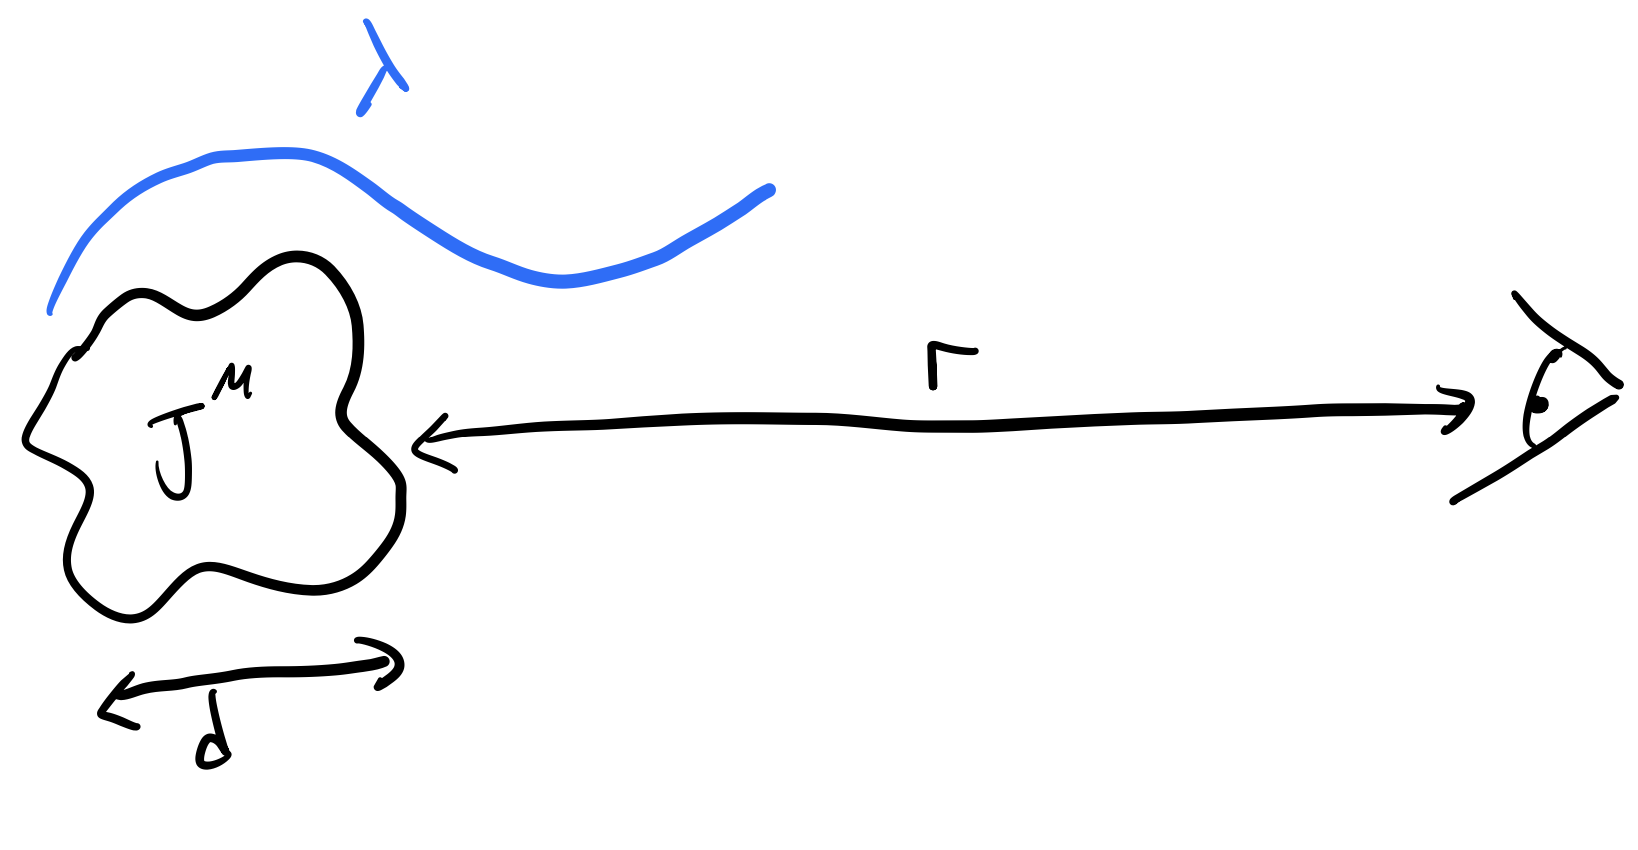
\includegraphics[scale=0.35]{Lectures/Images/lec10-lambdard.png}
\end{center}

Because we have only so much time, we assume $d \ll \lambda$. There are then two limits to consider, the near-field region $d \ll r \ll \lambda$ and the far-field region $d \ll \lambda \ll r$ (the intermediate cases are the most complicated):

\begin{center}
    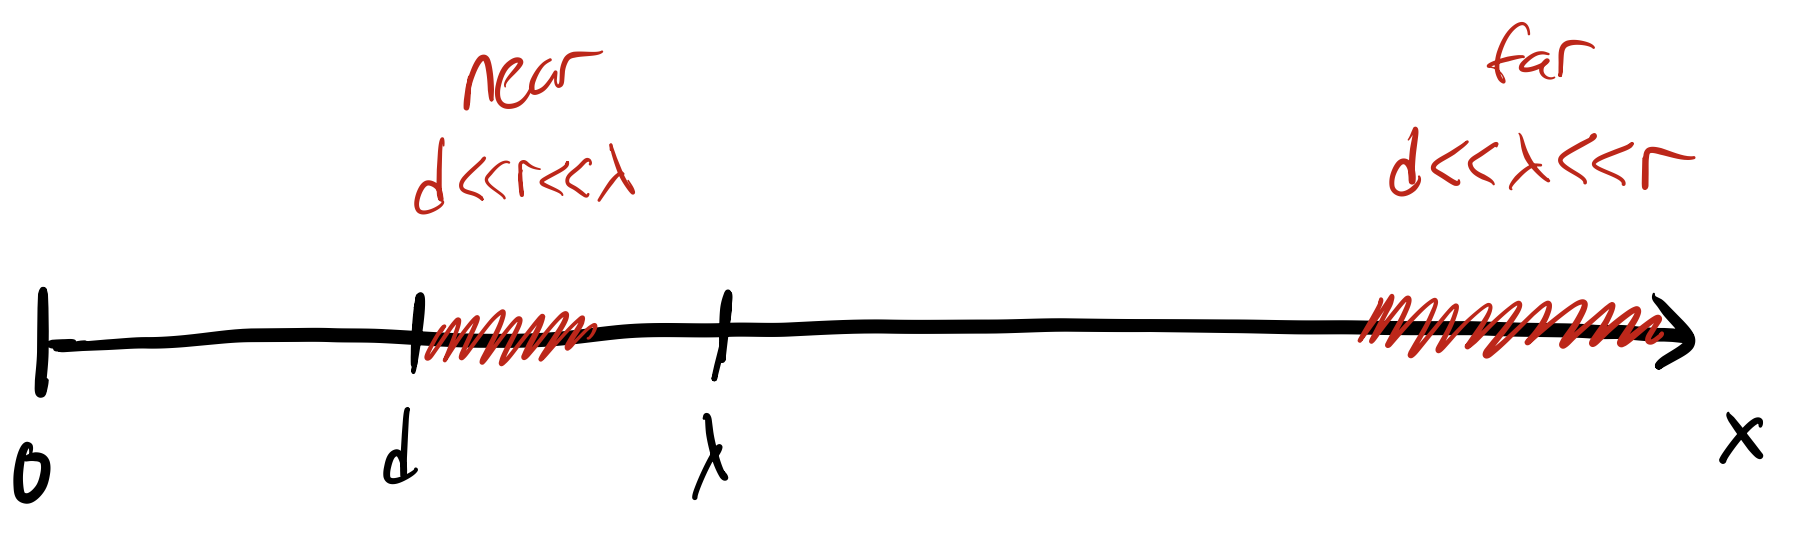
\includegraphics[scale=0.35]{Lectures/Images/lec10-nearfar.png}
\end{center}

In the near-field region, $e^{ik\abs{\v{x} - \v{x}'}} \approx 1$, because $\abs{\v{x} - \v{x}'}$ never goes to scales above $\lambda$. In this limit, the integral becomes simple:
\begin{equation}
    \v{A}(\v{x}) = \frac{\mu_0}{4\pi}\int d^3\v{x}'\frac{\v{J}(\v{x'})}{\abs{\v{x} - \v{x}'}}
\end{equation}
which is the static case which you studied in PHYS 322. This limit is not interesting to us, because we are trying to study radiation from this source. What about the far-field limit? In this limit, we might want to say we can erase the $\v{x}'$ in the denominator and numerator. This is half right; we can omit it in the denominator, but not in the numerator. Let's see why this is.

\begin{center}
    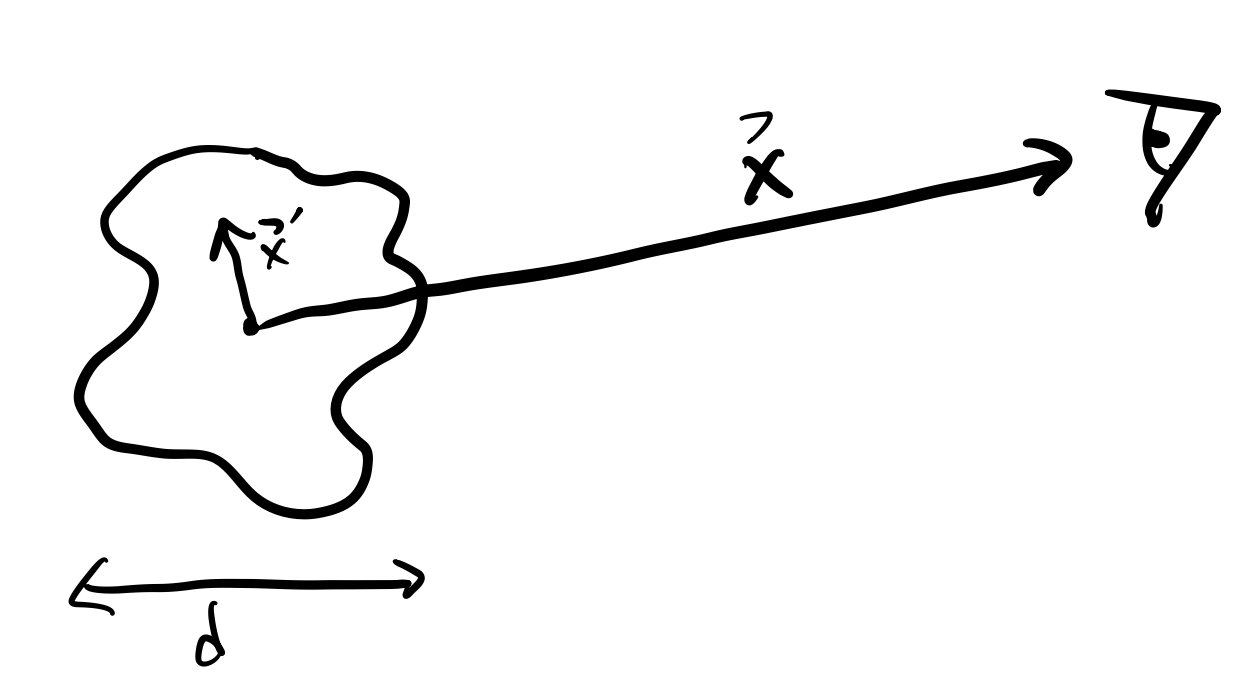
\includegraphics[scale=0.35]{Lectures/Images/lec10-rrprime.png}
\end{center}

Let's study $\abs{\v{x} - \v{x}'}^2$:
\begin{equation}
    \abs{\v{x} - \v{x}'} = \abs{\v{x}}^2 - 2\v{x} \cdot \v{x}' + \abs{\v{x}'}^2
\end{equation}
The last term can indeed be neglected as it is $O(d^2)$ while the other terms are $O(r^2), O(r)$; writing $\v{x} = r\hat{\v{n}}$, we have:
\begin{equation}
    \abs{\v{x} - \v{x}'}^2 \sim r^2 - 2r\hat{\v{n}} \cdot \v{x}' 
\end{equation}
and so:
\begin{equation}
    \abs{\v{x} - \v{x}'} = r - \hat{\v{n}} \cdot \v{x}' + O(\frac{1}{r})
\end{equation}
Then:
\begin{equation}
    \v{A}(\v{x}) = \frac{\mu_0}{4\pi}\frac{e^{ikr}}{r}\int d^3\v{x}' \v{J}(\v{x'})e^{-ik\hat{\v{n}}\cdot\v{x}'}
\end{equation}
The first observation; if we look at the prefactor $\frac{e^{ikr}}{r}$, we find that $\v{A} \sim \frac{1}{r}$, so $\v{E}, \v{B} \sim \frac{1}{r}$ and so the Poynting vector at leading order goes as $\frac{1}{r^2}$, which is the appropriate form for having finite radiation. Pictorially, it looks like an outgoing spherical wave. If we look at the second/integral term, this is $O(1)$ as there is no $r$ dependence. But, it is not negligible - it \emph{does} have angular dependence. The answer will depend on the direction we put our detector $\hat{\v{n}} = \hat{\v{n}}(\theta, \phi)$. Depending on the current distribution, we get different values for the angles $\theta, \phi$. Our task for next time is to finish analyzing this far-field result.